ネットワークではプロセス間はどのようにしてSocketを使って通信を行うのでしょうか?まず解決しなければならない問題はどのようにユニークなプロセスのひとつを認識するのかということです。そうでなければ通信を始めることすらままなりません!ローカルでプロセスPIDを使って一つのプロセスを識別します。実はTCP/IPプロトコル族ではすでにこの問題を解決してくれています。ネットワーク層の"ipアドレス"はネットワーク上のホストを一意に認識しており、トランスポート層の"プロトコル+ポート"はホストのアプリケーションプログラム(プロセス)を一意に認識することができます。これら3つの組み合わせ(ipアドレス、プロトコル、ポート)を利用することで、ネットワークのプロセスを認識することができます。ネットワークにおいて通信を行う必要のあるプロセスはこのタグを利用して互い通信を行うことができます。以下のTCP/IPプロトコルの構造図をご覧ください。

\begin{figure}[H]
  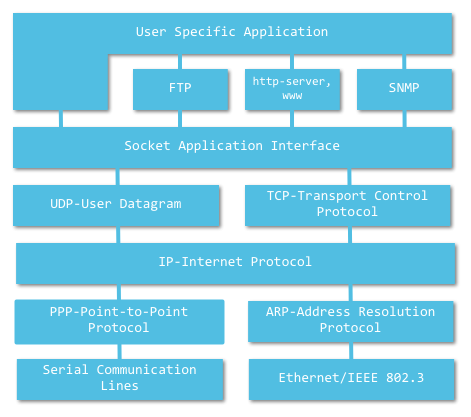
\includegraphics[width=14cm]{8.1.socket.png}
   \label{図8.1}
   \caption{七階層のネットワークプロトコルの図}
\end{figure}

TCP/IPプロトコルを使用したアプリケーションプログラムは通常アプリケーションプログラムのポートを採用します:UNIX BSDのソケット(socket)とUNIX System VのTLI(すでに淘汰されています)によってネットワークプロセス間の通信を実現します。現在ではほぼすべてのアプリケーションプログラムではsocketが採用されています。現在はネットワーク時代で、ネットワークのプロセス通信はどこにでも存在します。"すべてがSocket"というのはこういうことです。
